\documentclass[border = 1cm, preview, varwidth = \maxdimen]{standalone}

\usepackage{xeCJK}
\usepackage{ifthen}

% mathematics
\usepackage{amsmath}
\usepackage{amssymb}
\usepackage{derivative}
\derivset{\pdif}[style-notation=multiple]
\usepackage{esint}

% tikz
\usepackage{tikz}
\usepackage{tikz-cd}
\usetikzlibrary{arrows}
\usetikzlibrary{automata}
\usetikzlibrary{positioning}
\tikzset{->, > = stealth', node distance = 2cm}
\tikzcdset{arrow style = tikz}

\begin{document}

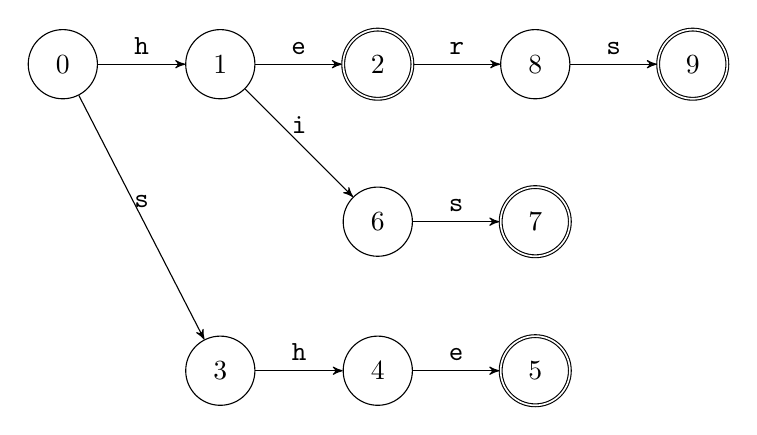
\begin{tikzpicture}
  % nodes
  \node (0) [state] {0};
  \node (1) [state, right of = 0] {1};
  \node (2) [state, accepting, right of = 1] {2};
  \node (3) [state, below = 3 of 1] {3};
  \node (4) [state, right of = 3] {4};
  \node (5) [state, accepting, right of = 4] {5};
  \node (6) [state, below of = 2] {6};
  \node (7) [state, accepting, right of = 6] {7};
  \node (8) [state, right of = 2] {8};
  \node (9) [state, accepting, right of = 8] {9};
  % edges
  \draw (0) edge [above] node {\tt h} (1);
  \draw (0) edge [above] node {\tt s} (3);
  \draw (1) edge [above] node {\tt e} (2);
  \draw (1) edge [above] node {\tt i} (6);
  \draw (2) edge [above] node {\tt r} (8);
  \draw (3) edge [above] node {\tt h} (4);
  \draw (4) edge [above] node {\tt e} (5);
  \draw (6) edge [above] node {\tt s} (7);
  \draw (8) edge [above] node {\tt s} (9);
\end{tikzpicture}

\end{document}
